%------------%
%  Preamble  %
%------------%

\documentclass[final,11pt]{article}
\usepackage[paperwidth=9.0in, top=1.2in, bottom=1.2in, left=1.2in, right=1.2in]{geometry}
\usepackage{amsmath}
\usepackage{color}
\usepackage{multirow}
\usepackage{setspace}
\usepackage{fancyhdr}
\usepackage{longtable}
\usepackage{array}
\usepackage{booktabs}
\usepackage{mathpazo}
\usepackage{threeparttable}
\usepackage{eurosym}
\usepackage{graphicx}
\usepackage[colorlinks, linkcolor=blue, anchorcolor=blue, citecolor=blue]{hyperref}

\usepackage[colorlinks, linkcolor=blue, anchorcolor=blue, citecolor=blue]{hyperref}

\renewcommand{\headrulewidth}{0pt}
\setlength{\arraycolsep}{10pt}
\setlength\headheight{0.5cm}
\setlength\headsep{0.8cm}
\setlength\footskip{1.0cm}
\setlength{\parindent}{0em}
\pagestyle{fancy}
\chead{\textcolor[rgb]{0.5,0.5,0.5}{\sc Spring 2025: ECON 6100}}

%------------%
%  Document  %
%------------%

\begin{document}
\thispagestyle{empty}
\begin{spacing}{1.25}

\textbf{Your Name: Po Yu Chen\hfill Problem Set 1 Due: Feb. 18, 2025}\\

(1) The Poisson distribution has probability mass function
\begin{gather}
    p(y_i|\theta)=\frac{\theta^{y_i}e^{-\theta}}{y_i!},\qquad \theta>0,\qquad y_i=0,1,\ldots
\end{gather}
and let $y_1,\ldots,y_n$ be random sample from this distribution.
\begin{enumerate}
    \item Show that the gamma distribution $\mathcal{G}(\alpha,\beta)$ is a conjugate prior distribution for the Poisson distribution.
    \item Show that $\bar{y}$ is the MLE for $\theta$.
    \item Write the mean of the posterior distribution as a weighted average of the mean of the prior distribution and the MLE.
    \item What happens to the weight on the prior mean as $n$ becomes large?
\end{enumerate}

{
\textbf{Solution:}
\begin{enumerate}
    %-------------------------------------------%
    \item \textbf{Show that the Gamma distribution $G(\alpha, \beta)$ is a conjugate prior for the Poisson distribution.}

    The Gamma prior is given by
    \begin{gather}
        \pi(\theta \mid \alpha, \beta) \;\propto\; \theta^{\alpha - 1} \, e^{-\tfrac{\theta}{\beta}}.
    \end{gather}
    The likelihood function for $n$ observations $\begin{bmatrix} y_1 \\ y_2 \\ \vdots \\ y_n \end{bmatrix}$ from $\text{Poisson}(\theta)$ is
    \begin{gather}
        f\!\Bigl(\begin{bmatrix} y_1 \\ y_2 \\ \vdots \\ y_n \end{bmatrix} \,\Big|\ \theta\Bigr)
        \;\propto\;
        \theta^{\sum y_i}\,e^{-\,\theta\,n}.
    \end{gather}
    Hence, by Bayes' theorem, the posterior distribution is
    \begin{gather}
    f(    \theta | 
    \begin{bmatrix}
    y_1 \\
    y_2 \\
    \vdots \\
    y_n \\
    \end{bmatrix}) \propto \theta^{\alpha - 1 + \sum y_i}e^{-{\theta(\frac{1}{\beta} + n)}}
     \end{gather}

    \paragraph{2.1 Likelihood and log-likelihood.}
    For $n$ i.i.d.\ observations, the likelihood $L(\theta)$ is
    \[
    L(\theta \,\mid\, y_1, \dots, y_n)
    \;=\;
    \prod_{i=1}^n \frac{\theta^{y_i} e^{-\theta}}{y_i!}
    \;=\;
    \frac{\theta^{\sum_{i=1}^n y_i}\; e^{-n \theta}}{\prod_{i=1}^n y_i!}.
    \]
    The log-likelihood $\ell(\theta)$ is
    \[
    \ell(\theta)
    \;=\;
    \log L(\theta \,\mid\, y_1, \dots, y_n)
    \;=\;
    \sum_{i=1}^n \bigl(y_i \log \theta \;-\; \theta \;-\; \log y_i!\bigr)
    \;=\;
    \Bigl(\sum_{i=1}^n y_i\Bigr)\,\log \theta 
    \;-\;
    n\,\theta
    \;-\;
    \sum_{i=1}^n \log y_i!.
    \]
    Since $\sum_{i=1}^n \log y_i!$ does not depend on $\theta$, it can be treated as a constant.

    \paragraph{2.2 Maximizing $\ell(\theta)$.}
    Taking the derivative of $\ell(\theta)$ w.r.t.\ $\theta$ and setting it to zero:
    \[
    \frac{d}{d\theta}\,\ell(\theta)
    \;=\;
    \frac{\sum_{i=1}^n y_i}{\theta}
    \;-\;
    n
    \;=\;
    0,
    \]
    which implies
    \[
      \frac{\sum_{i=1}^n y_i}{\theta} \;=\; n
      \quad\Longrightarrow\quad
      \hat{\theta}_{\mathrm{MLE}}
      \;=\;
      \frac{1}{n} \sum_{i=1}^n y_i
      \;=\;
      \bar{y}.
    \]
    Thus, the \textbf{MLE} for $\theta$ is the sample mean $\bar{y}$.

    \paragraph{3.1 Posterior distribution.}
    We already found that, under a $\mathrm{Gamma}(\alpha, \beta)$ prior and Poisson$(\theta)$ likelihood,
    \[
      \theta 
      \,\Big|\,
      \begin{bmatrix}y_1 \\ y_2 \\ \vdots \\ y_n\end{bmatrix}
      \;\sim\;
      \mathrm{Gamma}\!\Bigl(\alpha + \sum_{i=1}^n y_i,\;\beta + n\Bigr).
    \]

    \paragraph{3.2 Posterior mean as a weighted average.}
    The mean of a $\mathrm{Gamma}(a, b)$ distribution is $a / b$. Therefore, the posterior mean is
    \[
    \mathbb{E}[\theta \mid y_1,\dots,y_n]
    \;=\;
    \frac{\alpha + \sum_{i=1}^n y_i}{\beta + n}.
    \]
    Recognize that
    \[
    \alpha + \sum_{i=1}^n y_i
    \;=\;
    \beta\,\Bigl(\tfrac{\alpha}{\beta}\Bigr)
    \;+\;
    n\,\Bigl(\tfrac{\sum_{i=1}^n y_i}{n}\Bigr).
    \]
    Hence, if we let $\tfrac{\alpha}{\beta}$ be the prior mean and $\bar{y} = \tfrac{1}{n}\sum_{i=1}^n y_i$ the MLE (sample mean), then
    \[
    \frac{\alpha + \sum_{i=1}^n y_i}{\beta + n}
    \;=\;
    \frac{\beta}{\beta + n}\,\Bigl(\tfrac{\alpha}{\beta}\Bigr)
    \;+\;
    \frac{n}{\beta + n}\,\bar{y}.
    \]
    Thus, the posterior mean is a \emph{weighted average}:
    \[{
    \mathbb{E}[\theta \mid y_1,\dots,y_n]
    \;=\;
    \Bigl(\tfrac{\beta}{\beta + n}\Bigr)\,
    \Bigl(\tfrac{\alpha}{\beta}\Bigr)
    \;+\;
    \Bigl(\tfrac{n}{\beta + n}\Bigr)\,\bar{y}.
    }
    \]

    \paragraph{4.1 n becomes large}
    From the expression
\[
\mathbb{E}[\theta \mid y_1,\dots,y_n]
\;=\;
\frac{\beta}{\beta + n}\,\left(\frac{\alpha}{\beta}\right)
\;+\;
\frac{n}{\beta + n}\,\bar{y},
\]
the weight on the \emph{prior mean} $\frac{\alpha}{\beta}$ is $\frac{\beta}{\beta + n}$. As $n \to \infty$,
\[
\frac{\beta}{\beta + n}
\;\longrightarrow\;
0.
\]
Therefore, for large sample size, the posterior mean is dominated by the sample mean $\bar{y}$, reflecting the fact that the data overwhelms the prior information when $n$ is very large.

\end{enumerate}
}
\newpage 


(2) Consider the following two sets of data obtained after tossing a die 100 and 1000 times, respectively:
\begin{center}
    \begin{tabular}{ r r r r r r r }
        \hline
        $n$ & 1 & 2 & 3 & 4 & 5 & 6 \\
        \hline
        100 & 19 & 12 & 17 & 18 & 20 & 14 \\  
        1000 & 190 & 120 & 170 & 180 & 200 & 140 \\
        \hline
    \end{tabular}
\end{center}
Suppose you are interested in $\theta_1$, the probability of obtaining a one spot. Assume your prior for all the probabilities is a Dirichlet distribution, where each $\alpha_i=2$. Compute the posterior distribution for $\theta_1$ for each of the sample sizes in the table. Plot the resulting distribution and compare the results. Comment on the effect of having a larger sample.

\section*{Solution}


We have a (fair or unfair) six-sided die and a prior distribution over its face--landing probabilities 
\[
(\theta_1, \theta_2, \theta_3, \theta_4, \theta_5, \theta_6)
\]
given by a Dirichlet distribution with parameters \(\alpha_i = 2\) for \(i=1,2,\ldots,6\). That is,
\[
(\theta_1,\ldots,\theta_6) \sim \text{Dirichlet}(\alpha_1,\ldots,\alpha_6), 
\quad\text{where}\quad \alpha_1 = \alpha_2 = \cdots = \alpha_6 = 2.
\]

We then observe two different datasets:

\begin{enumerate}
    \item After rolling the die 100 times, we obtain the counts 
    \[
    n_1 = 19,\quad n_2 = 12,\quad n_3 = 17,\quad n_4 = 18,\quad n_5 = 20,\quad n_6 = 14.
    \]
    \item After rolling the die 1000 times, we obtain the counts 
    \[
    n_1 = 190,\quad n_2 = 120,\quad n_3 = 170,\quad n_4 = 180,\quad n_5 = 200,\quad n_6 = 140.
    \]
\end{enumerate}

We are specifically interested in the posterior distribution of \(\theta_1\), the probability of obtaining a one-spot, for each sample size. We will compute the posterior distributions and compare them.

\subsection*{Posterior Distribution}

Given a Dirichlet prior 
\[
(\theta_1,\ldots,\theta_6) \sim \text{Dirichlet}(\alpha_1, \ldots, \alpha_6)
\]
and observed counts 
\[
(n_1,\ldots,n_6),
\]
the posterior distribution is 
\[
(\theta_1,\ldots,\theta_6) \mid \text{data} \sim \text{Dirichlet}(\alpha_1 + n_1, \ldots, \alpha_6 + n_6).
\]
The marginal distribution of any one component, say \(\theta_1\), from a 
\(\text{Dirichlet}(\gamma_1,\gamma_2,\ldots,\gamma_6)\) is 
\[
\theta_1 \sim \text{Beta}\!\bigl(\gamma_1,\,\gamma_2+\gamma_3+\cdots+\gamma_6\bigr).
\]

\subsubsection*{Case 1: 100 Rolls}

\paragraph{Data:} \((n_1,n_2,n_3,n_4,n_5,n_6) = (19,12,17,18,20,14)\).

\paragraph{Prior:} \(\alpha_i = 2\) for each \(i\).

\paragraph{Posterior Parameters:}
\[
\alpha_1 + n_1 = 2 + 19 = 21,
\]
\[
\sum_{j=2}^6 (\alpha_j + n_j) \;=\; \sum_{j=2}^6 (2 + n_j)
\;=\; 5 \times 2 + (12 + 17 + 18 + 20 + 14)
\;=\; 10 + 81
\;=\; 91.
\]

Hence,
\[
\theta_1 \mid \text{data}_{100} 
\;\sim\; \text{Beta}(21,\,91).
\]

\paragraph{Summary for 100 Rolls:}
\[
\theta_1 \sim \text{Beta}(21,91), 
\]
which has mean 
\(\displaystyle \frac{21}{21 + 91} = \frac{21}{112} \approx 0.1875.\)

\subsubsection*{Case 2: 1000 Rolls}

\paragraph{Data:} \((n_1,n_2,n_3,n_4,n_5,n_6) = (190,120,170,180,200,140)\).

\paragraph{Prior:} \(\alpha_i = 2\) for each \(i\).

\paragraph{Posterior Parameters:}
\[
\alpha_1 + n_1 = 2 + 190 = 192,
\]
\[
\sum_{j=2}^6 (\alpha_j + n_j) \;=\; \sum_{j=2}^6 (2 + n_j)
\;=\; 5 \times 2 + (120 + 170 + 180 + 200 + 140)
\;=\; 10 + 810
\;=\; 820.
\]

Hence,
\[
\theta_1 \mid \text{data}_{1000} 
\;\sim\; \text{Beta}(192,\,820).
\]

\paragraph{Summary for 1000 Rolls:}
\[
\theta_1 \sim \text{Beta}(192,820), 
\]
which has mean 
\(\displaystyle \frac{192}{192 + 820} = \frac{192}{1012} \approx 0.1896.\)

\subsection*{Plots and Comparison}

\begin{figure}[h!]
    \centering
        \centering
        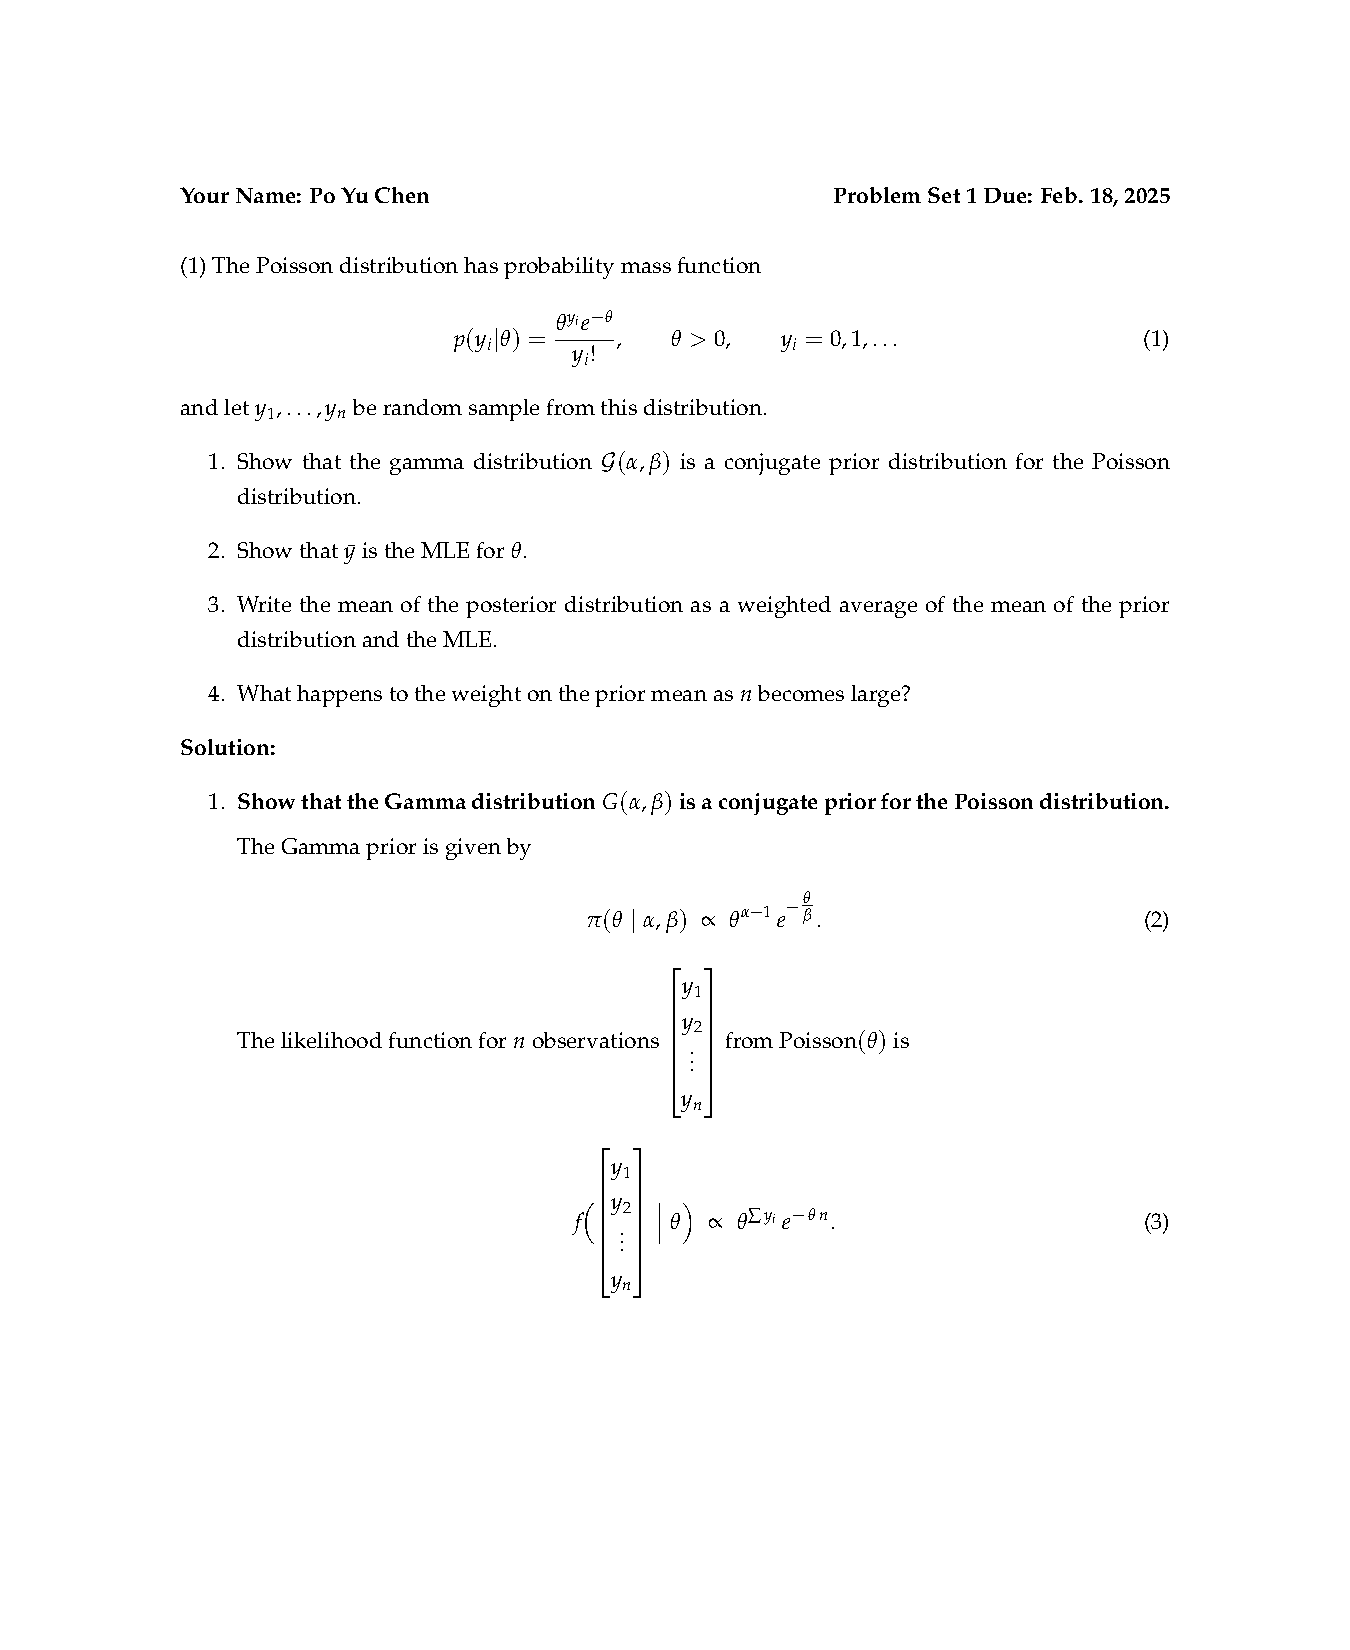
\includegraphics[width=0.7\textwidth]{PS1.png}
    \caption{Posterior distributions of \(\theta_1\) based on 100 rolls (Beta(21,91)) and 1000 rolls (Beta(192,820)).}
    \label{fig:posterior_plots}
\end{figure}

\noindent
\textbf{Observations:}

\begin{itemize}
    \item The posterior after 100 rolls, \(\text{Beta}(21,91)\), is more spread out compared to the posterior after 1000 rolls, \(\text{Beta}(192,820)\). 
    \item As the sample size increases, the posterior distribution concentrates more sharply around its mean, reflecting higher confidence in the estimate of \(\theta_1\).
    \item Both posterior means are close to the empirical frequency of rolling a one , but the distribution for the larger sample size is noticeably narrower.
\end{itemize}

\subsection*{Conclusion}

With a larger sample size (1000 vs. 100 rolls), the posterior distribution for \(\theta_1\) becomes more sharply peaked around the observed proportion of ones. This illustrates the general Bayesian principle that the posterior becomes more concentrated as the amount of observed data increases, reducing uncertainty about the parameter \(\theta_1\).

\end{spacing}
\end{document}